\chapter{Improved porosimetric techniques for highly ultramicroporous carbons}
\label{ch:dual_isotherm}

\newpage
\section*{Abstract}
It has been shown both in recent literature, and according to the work in chapters \ref{ch:cbs} and \ref{ch:impregnation} that porosimetry based on \ce{N2} isotherms at \qty{-196}{\degreeCelsius} is insufficient for the precise analysis of porosity in ultramicroporous carbons. This is a result of both \ce{N2}'s high quadrupole moment as well as its poor diffusion into \glspl{ultramicropore}. The investigation of alternative \glspl{adsorbate} for these materials, in particular \ce{H2} and \ce{O2} has shown some promise in this regard, and the development of the dual isotherm fitting method allows for a unified \acrshort{psd} to be determined with this method. As such this chapter investigates the relative utility of the simultaneous fitting of \ce{O2}/\ce{H2} isotherms to \acrfull{nldft} kernels in determining porosity of carbons found in this work, as compared to dual isotherm \ce{N2}/\ce{H2} as well as to single isotherm \acrshort{nldft} porosimetry and classical methods such as \acrshort{bet}. 

It was found that the \ce{O2}/\ce{H2} method provides an extremely high level of detail in the differences in porosity of carbons activated with differing amounts of \gls{porogen}. That is, not only can overall changes in porosity be observed, but more significantly very small changes in pore width are observable with this technique. The latter cannot be achieved using dual isotherm \ce{N2}/\ce{H2} fitting, or indeed by any other means investigated in this work. As a result, \ce{O2}/\ce{H2} analysis provides hints at pore formation mechanisms in these types of porous carbons that are not evident according to \ce{N2}/\ce{H2} analysis. Furthermore, it is apparent that the use of the \ce{H2} isotherm provides knowledge of porosity in the small \gls{ultramicropore} region which is inaccessible to either of the larger probes, \ce{O2} or \ce{N2}. Finally, the \acrshort{nldft} methodology used in this work provides quite different understanding of the variation of apparent surface area with synthetic conditions as compared to the traditional \acrshort{bet} method, which is likely a result of the greater suitability of the \acrshort{nldft} kernel to the analysis of ultramicroporous \glspl{turbostratic carbon} examined herein.
 
\newpage
\section{Introduction}
\label{s:dual_intro}

\begin{figure}[b!]
    \centering
    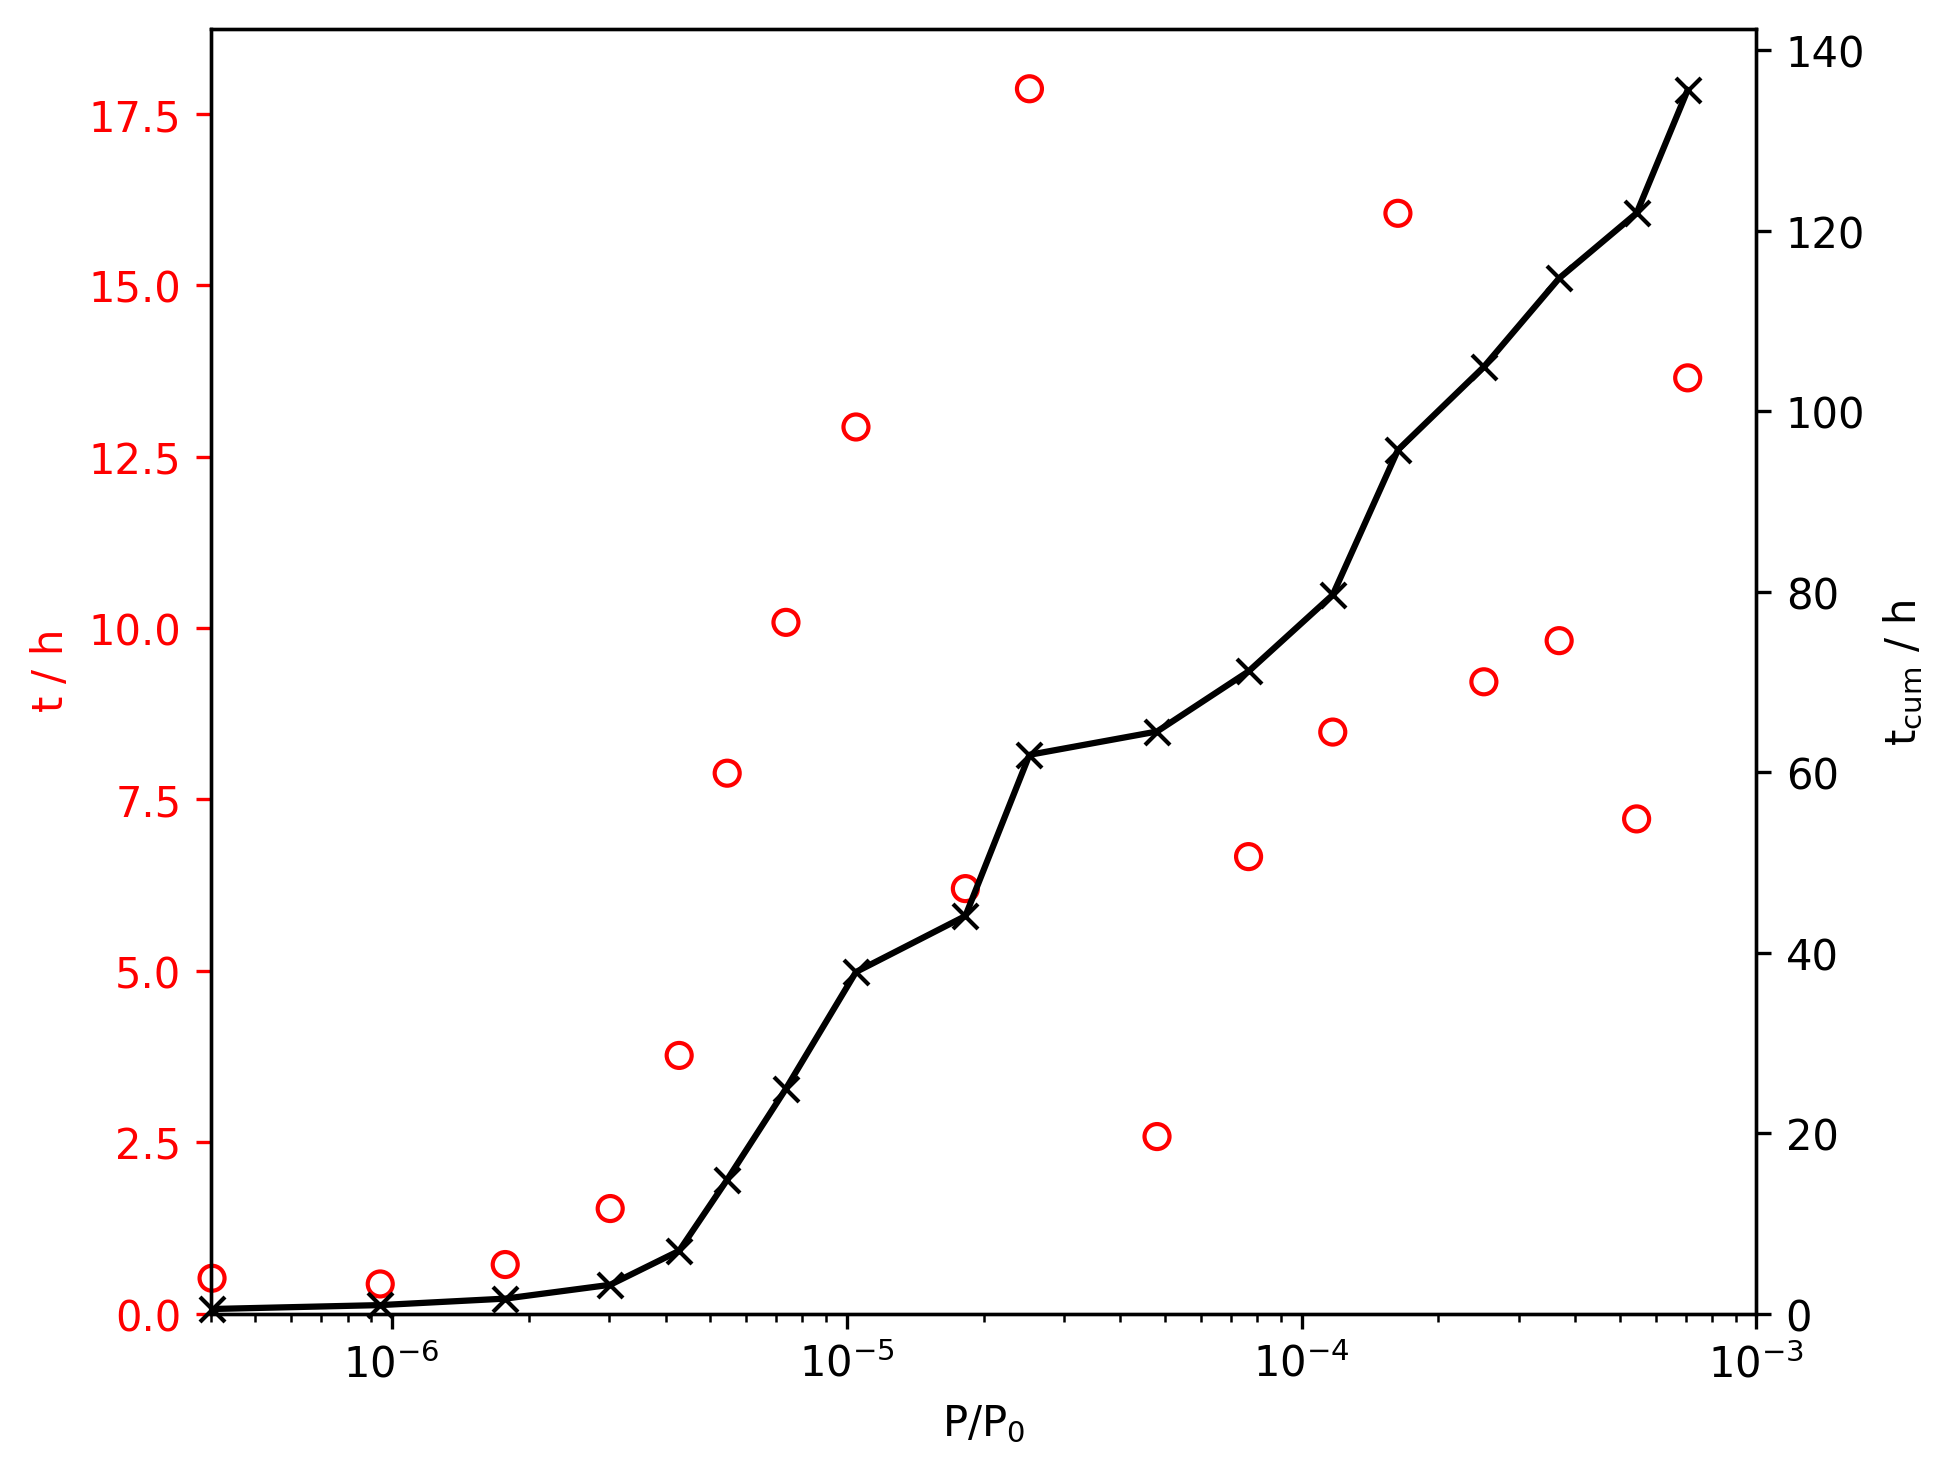
\includegraphics[width=0.95\columnwidth,keepaspectratio]{5-dual_isotherm/figs/timings.png}
    \caption{An example of the egregiously long equilibration times for individual points, $t$ and cumulative analysis time, $t_{cum}$ in the measurement of an \ce{N2} isotherm at \qty{-196}{\degreeCelsius} on sample hD-0700. The isotherm only reached a $P/P_0$ of $10^{-3}$ before being cancelled by the instrument.}
    \label{fig:timings}
\end{figure}

In chapters \ref{ch:cbs} and \ref{ch:impregnation}, it became clear that derivation of \acrshortpl{psd} and related porosimetric values from the typical \ce{N2} (\qty{-196}{\degreeCelsius}) isotherm was not sufficiently accurate. In particular, for carbons with a low degree of activation isotherm measurement became impractical due to extremely long equilibration times - see \ref{pub:dual_iso} \textbf{section 3.1.}, and figure \ref{fig:timings}. In many cases this resulted in limited isotherms that do not include points at ultra-low pressures ($P/P_0 < 10^{-4}$) as shown in figures \ref{fig:0TTT_psdisofull}, \ref{fig:NCxx-600_psdisofull}-\ref{fig:NCxx-800_psdisofull}. \acrshort{psd}s from these incomplete and/or poorly equilibrated isotherms indicate a high degree of porosity in the \gls{ultramicropore} region, however \glspl{ultramicropore} fill at ultra-low pressures. Thus, as noted in previous chapters there can be very minimal confidence in the results derived from this technique. This issue has been reported as early as 1982.\citep{RodriguezReinoso1982Activated} A solution in the literature to this problem has been to employ \ce{CO2} isotherms at \qty{0}{\degreeCelsius} in order to probe \glspl{ultramicropore} and small \glspl{supermicropore}.\citep{Jagiello2004Comparison, Jagiello2015Dual, Garrido1987Use, LozanoCastello2004Usefulness} The porosity up to some upper-limit (usually taken as somewhere around \qty{10}{\angstrom}) can then be calculated.\citep{furimsky2000characterization, sing1989use} \acrshort{psd}s have also been calculated from these isotherms,\citep{Jagiello2004Comparison} and indeed Jagiello and co-workers have developed techniques to fit \acrshort{nldft} kernels simultaneously to \ce{CO2} and \ce{N2} isotherms.\citep{Jagiello2019Enhanced, Jagiello2015Dual} However, in the case of \glspl{turbostratic carbon}, the effect of the quadrupole moment of both \ce{CO2} and \ce{N2} on the accuracy of the resultant \acrshort{psd} means that the much less polar \ce{H2} and \ce{O2} are now becoming common replacements to elucidate the full porosity of such materials.\citep{Jagiello2020Exploiting, Blankenship2022Confirmation, GrauMarin2020Evaluation} Furthermore, \ce{O2} and \ce{H2} isotherms can be measured at \qty{-196}{\degreeCelsius}, unlike \ce{CO2} which is solid at this temperature - thus eliminating the need to change temperature control apparatus. Therefore, this chapter investigates the relative utility of both \ce{N2}/\ce{H2} and \ce{O2}/\ce{H2} pairs in determining \acrshortpl{psd} of the ultramicroporous carbons produced in chapters \ref{ch:cbs} and \ref{ch:impregnation}.

\subsection{The 2D-NLDFT-HS kernel}
\label{ss:2d-nldft-hs}
Section \ref{sss:dft} explained the general process of determining \acrshort{dft} kernels, and then fitting them to an experimental isotherm in order to determine the \acrshort{psd}. The earliest kernels for \gls{adsorption} of \ce{N2} on porous carbon used a one-dimensional, homogeneous, semi-infinte model of the pore wall surface.\citep{seaton1989new} That is, the pore wall is completely flat and its length extends to infinity. This simplified kernel determination as pore space was only characterised by the pore width, and used a local density approximation to account for repulsive forces; short-range interactions are omitted for simplicity. Unfortunately this results in a poor description of the density profile of \gls{adsorbate} molecules near the pore walls. Tarazona and co-workers improved on this model by considering these short-range interactions, producing the so-called \acrfull{nldft} kernel.\citep{tarazona1985free, tarazona1987phase} This nonetheless does not consider the energetic and chemical heterogeneity of pore walls within real porous carbons. Not only is this inaccurate, but the use of these kernels leads to poor fitting to the experimental isotherm and consistent artefacts in the resultant \acrshort{psd}.\citep{Jagiello20132D,  olivier1998improving, lueking2009tests, nguyen2004characterization} Olivier suggested applying weightings to the model isotherms used when fit to the experimental data as well as using a finite pore model,\citep{olivier1998improving} while Nguyen and Bhatia found some improvements by considering pore wall heterogeneity by varying the pore wall thickness.\citep{nguyen2004characterization} Jagiello \textit{et al.}, however consider the pore wall to be a two-dimensional surface, having regular sinusoidal corrugations. This accounts for both chemical and energetic heterogeneity\citep{Jagiello20132D} and the eponymous 2D-NLDFT-HS (2-dimensional NLDFT heterogeneous surface) approach results in a better fit to the experimental isotherm.\citep{Jagiello20132D, puziy2016comparison, shi2021current} Thus far, the 2D-NLDFT-HS kernel has been developed for \ce{N2}, \ce{O2}, \ce{H2}, \ce{CO2}, and \ce{Ar}.\citep{Jagiello20132D, Jagiello2013, jagiello2019consistency, Jagiello2020Exploiting}

\subsection{Multiple isotherm fitting}
\label{ss:multi_iso}
The general \gls{adsorption} integral integral equation was is shown in section \ref{sss:dft}, equation \ref{eq:GAI}. For convenience, it is reproduced in equation \ref{eq:GAI_jagiello} in a form more useful to compare to calculations performed when fitting the \acrshort{dft} kernels to multiple isotherms simultaneously. $V(p_i)$ and $K(p_i,\,w)$ are the experimental isotherm and kernel respectively, and $f(w)$ is the differential \acrshort{psd} to be calculated.

\begin{equation} \label{eq:GAI_jagiello}
    V(p_i) = \int_{w_{min}}^{w_{max}} K(p_i,w) f(w) \, \mathrm{d}w
\end{equation}

The solution to this equation is quite involved, but is achievable using a method developed by Jagiello.\citep{Jagiello1994Stable} In short, a stable \acrshort{psd} can be determined by using the regularization approach to determine an appropriate fitting parameter, $\lambda$\citep{Hansen2001, Hansen1993use, Hansen2001L} and the discrete result is interpolated using the B-spline approach.\citep{knott2000interpolating, prautzsch2002bezier, deboor1978practical} This method is automated in the SAIEUS (Solution to the Adsorption Integral Equation Using Splines) program.\citep{Jagiello1994Stable} The $\lambda$ variable is added to the expression in equation \ref{eq:GAI_jagiello} to produce \ref{eq:GAI_jagiello_lambda};

\begin{equation} \label{eq:GAI_jagiello_lambda}
    V(p_i) = \int_{w_{min}}^{w_{max}} K(p_i,w) f(w) \, \mathrm{d}w + \lambda\int_{w_{min}}^{w_{max}}\left[ f''(w) \right]^2\, \mathrm{d}w
\end{equation}

When considering $M$ multiple isotherms, a summative approach is needed.\citep{caguiat2014uncertainties} Minimisation of the multi-isotherm, multi-kernel  expression in equation \ref{eq:multiple_isotherm} for each \gls{adsorbate}, $m$ will yield a single \acrshort{psd} for all $M$ isotherms.\footnote{The summative expression in equation \ref{eq:multiple_isotherm} is a result of the solution to the single isotherm general \gls{adsorption} integral equation described in equation \ref{eq:GAI_jagiello_lambda}. Its derivation is discussed by Jagiello in the original paper,\citep{Jagiello1994Stable} but is outside the scope of this work.}

\begin{equation} \label{eq:multiple_isotherm}
    \mathrm{min}\sum_{m}^{M}\sum_{i}^{N_m}\left[ V_m(p_i) - \int_{w_{min}}^{w_{max}}K_m(p_i,\,w)f(w)\,\mathrm{d}w\right]^2 + \lambda\int_{w_{min}}^{w_{max}}\left[ f''(w) \right]^2\, \mathrm{d}w
\end{equation}

Where $V_m(p_i)$ and $K_m(p_i,\,w)$ are the $m$th experimental isotherm and $m$th kernel respectively.\citep{Jagiello2015Dual, Jagiello2008Characterization, Jagiello2007}

\section[Exploring alternative porosimetric adsorbates]{Exploring alternative porosimetric \glspl{adsorbate}}
\label{s:dual_initial}
Section \ref{s:dual_intro} laid out the need to explore alternative porosimetric techniques for analysis of the ultramicroporous carbons produced in previous chapters. While a comprehensive comparison of dual fitting to \ce{N2}/\ce{H2} and \ce{O2}/\ce{H2} isotherm pairs is detailed in \ref{pub:dual_iso}, what follows here are the results of some initial analytical experiments using \ce{N2} and \ce{O2}, and combined \ce{O2}/\ce{H2} isotherms.

\subsection{Classical porosity}

While the purpose of this chapter is to use more advanced, \acrshort{nldft} techniques in the determination of porosity from \gls{physisorption} isotherms, comparing the classical measures of surface area and pore volume yielded by \ce{N2} and \ce{O2} isotherms at \qty{-196}{\degreeCelsius} also gives some interesting insights. Results of these analyses are displayed in table \ref{tb:n2_o2_classical}. The important distinctions between these \glspl{adsorbate} are their molecular cross-sectional areas ($\sigma$), kinetic diameters ($d_k$) and quadrupole moments ($\mu$). As stated before, \ce{O2} is significantly less polar than \ce{N2}, these \glspl{adsorbate} having $\mu$ of 0.155 and 0.697 respectively.\citep{Lide2007Handbook, Poling2001Properties, Graham1998Measurement} In terms of $d_k$ they are similar, and $\sigma_{O_2}$ is only slightly smaller than $\sigma_{N_2}$ at \qtylist[list-units=single]{0.143; 0.162}{\nm\squared}  respectively. However, it should be noted that there is no definitive, exact value for these $\sigma$ values as they vary according to the surface the molecule is being adsorbed onto.\citep{kodera1959molecular, kodera1960molecular, livingston1949cross} This variability is much more significant in the case of \ce{N2} due to its greater polarity - indeed $\sigma_{N_2}$ can vary for individual molecules of \ce{N2} on a single \gls{adsorbent} at different \gls{adsorption} sites.\citep{Jagiello2020Exploiting}

\begin{table}[ht!]
    \centering
    \caption{Comparison of classical measures of porosity derived using \ce{N2} and \ce{O2} porosimetry. $A_{BET}$ calculated using the Rouquerol method,\citep{Rouquerol2007Is} and $V_t$ using the single-point approach. Values in brackets indicate the microporous portion of surface area and pore volume as determined by t-plot using a Carbon Black STSA thickness curve. The two hD-0700 samples in table are repeat syntheses of the same sample. }
    \begin{tabularx}{\textwidth}{lXlXlXlXl}
    \toprule
        \textbf{Sample} & \multicolumn{4}{c}{$\mathbf{A_{BET}}$ \textbf{/ \unit[detect-weight]{\metre\squared\per\gram}}} &  \multicolumn{4}{c}{$\mathbf{V_t}$ \textbf{/ \unit[detect-weight]{\cm\cubed\per\gram}}} \\
        & \multicolumn{2}{c}{\textbf{\ce{N2}}} & \multicolumn{2}{c}{\textbf{\ce{O2}}} & \multicolumn{2}{c}{\textbf{\ce{N2}}} & \multicolumn{2}{c}{\textbf{\ce{O2}}} \\
    \midrule
        NC0.0-800 & 449 & (408) & 595 & (532) & 0.17 & (0.13) & 0.24 & (0.20) \\
        NC0.7-800 & 580 & (495) & 645 & (563) & 0.21 & (0.16) & 0.25 & (0.18) \\
        NC0.9-800 & 669 & (578) & 876 & (749) & 0.28 & (0.22) & 0.37 & (0.29) \\
        \\
        SA1.00-200 & 1410 & (1306) & 1513 & (1333) & 0.61 & (0.54) & 0.62 & (0.51)  \\
        \\
        SA0.00-250 & 949 & (838) & 596 & (514) & 0.18 & (0.16) & 0.25 & (0.20) \\
        SA0.50-250 & 906 & (826) & 1161 & (1066) & 0.51 & (0.47) & 0.40 & (0.34) \\
        SA1.00-250 & 1081 & (971) & 1266 & (1138) & 0.54 & (0.48) & 0.45 & (0.37) \\
        \\
        hD-0700\textit{(1)} & 278 & (242) & 428 & (355) & 0.18 & (0.11) & 0.16 & (0.12) \\
        hD-0700\textit{(2)} & 317 & (265) & 411 & (346) & 0.19 & (0.12) & 0.15 & (0.11) \\
    \bottomrule
    \end{tabularx}
    \label{tb:n2_o2_classical}
\end{table}

These issues with these classical analyses notwithstanding, the values for $A_{BET}$ derived from \ce{O2} porosimetry is generally higher than that from \ce{N2}. The relative percentage of surface area taken up by \glspl{micropore} is however consistent from both techniques, being between \qtylist[list-units=single]{83;92}{\percent} for all samples. On the other hand, $V_t$ does not show any consistency in the way it varies between the two techniques. It is likely that simply due to the large uncertainties in determination of pore volume \textit{via} the single-point method, any pattern is obscured. The increases in $A_{BET}$ found when using \ce{O2} at \qty{-196}{\degreeCelsius} as a molecular probe may indicate the ability of \ce{O2} to diffuse into pores inaccessible to \ce{N2}. It is also interesting to note that $A_{BET}$ is far more consistent for the two repeats of hD-0700 when determined using \ce{O2} rather than \ce{N2}, perhaps giving further indication of the improvements in reliability of results attained using this alternative \gls{adsorbate}. It is however difficult to categorically assert \ce{O2}'s superiority over \ce{N2} for this application from this evidence, due to the afforementioned problems with these classical techniques. 
%
\subsection{\texorpdfstring{Bimodal \acrshortpl{psd} from dual isotherm \ce{O2}/\ce{H2} analysis}{Bimodal PSD from dual isotherm O2/H2 analysis}}%

Initial investigations into dual isotherm analysis were for the purpose of comparing porosity as given by fitting of the 2D-NLDFT-HS kernel to \ce{N2} isotherms to that determined by the dual fitting of the appropriate 2D-NLDFT-HS kernels to \ce{O2} and \ce{H2} isotherms on carbon samples that appear to have a high proportion of \glspl{ultramicropore}. An example of this comparison is shown in figure \ref{fig:dual_psd_compare}. In general, it was found that the dual \ce{O2}/\ce{H2} fit yields greater overall porosity than the single isotherm fit. Furthermore, the \acrshort{psd}s are consistently bimodal for the dual isotherm fit. While \glspl{micropore} are typically subdivided at \qty{7.0}{\angstrom} into \glspl{ultramicropore} and \glspl{supermicropore} (as indicated by the dotted line in figure \ref{fig:dual_psd_compare}), the minimum between the two regions is at a consistently lower pore width than this. For this purpose, the pore volume ($V_{NLDFT}$) and surface area ($A_{NLDFT}$) are given in table \ref{tb:finepore} as subdivided into these two regions according to the variable local minimum ($w_{locmin}$). The separate regions appear to be a result of different probeable pore sizes of the two adsorptives - this issue is discussed in more depth in \ref{pub:dual_iso}, \textbf{section 3.3.1.}. 

\begin{figure}[hptb]
    \centering
    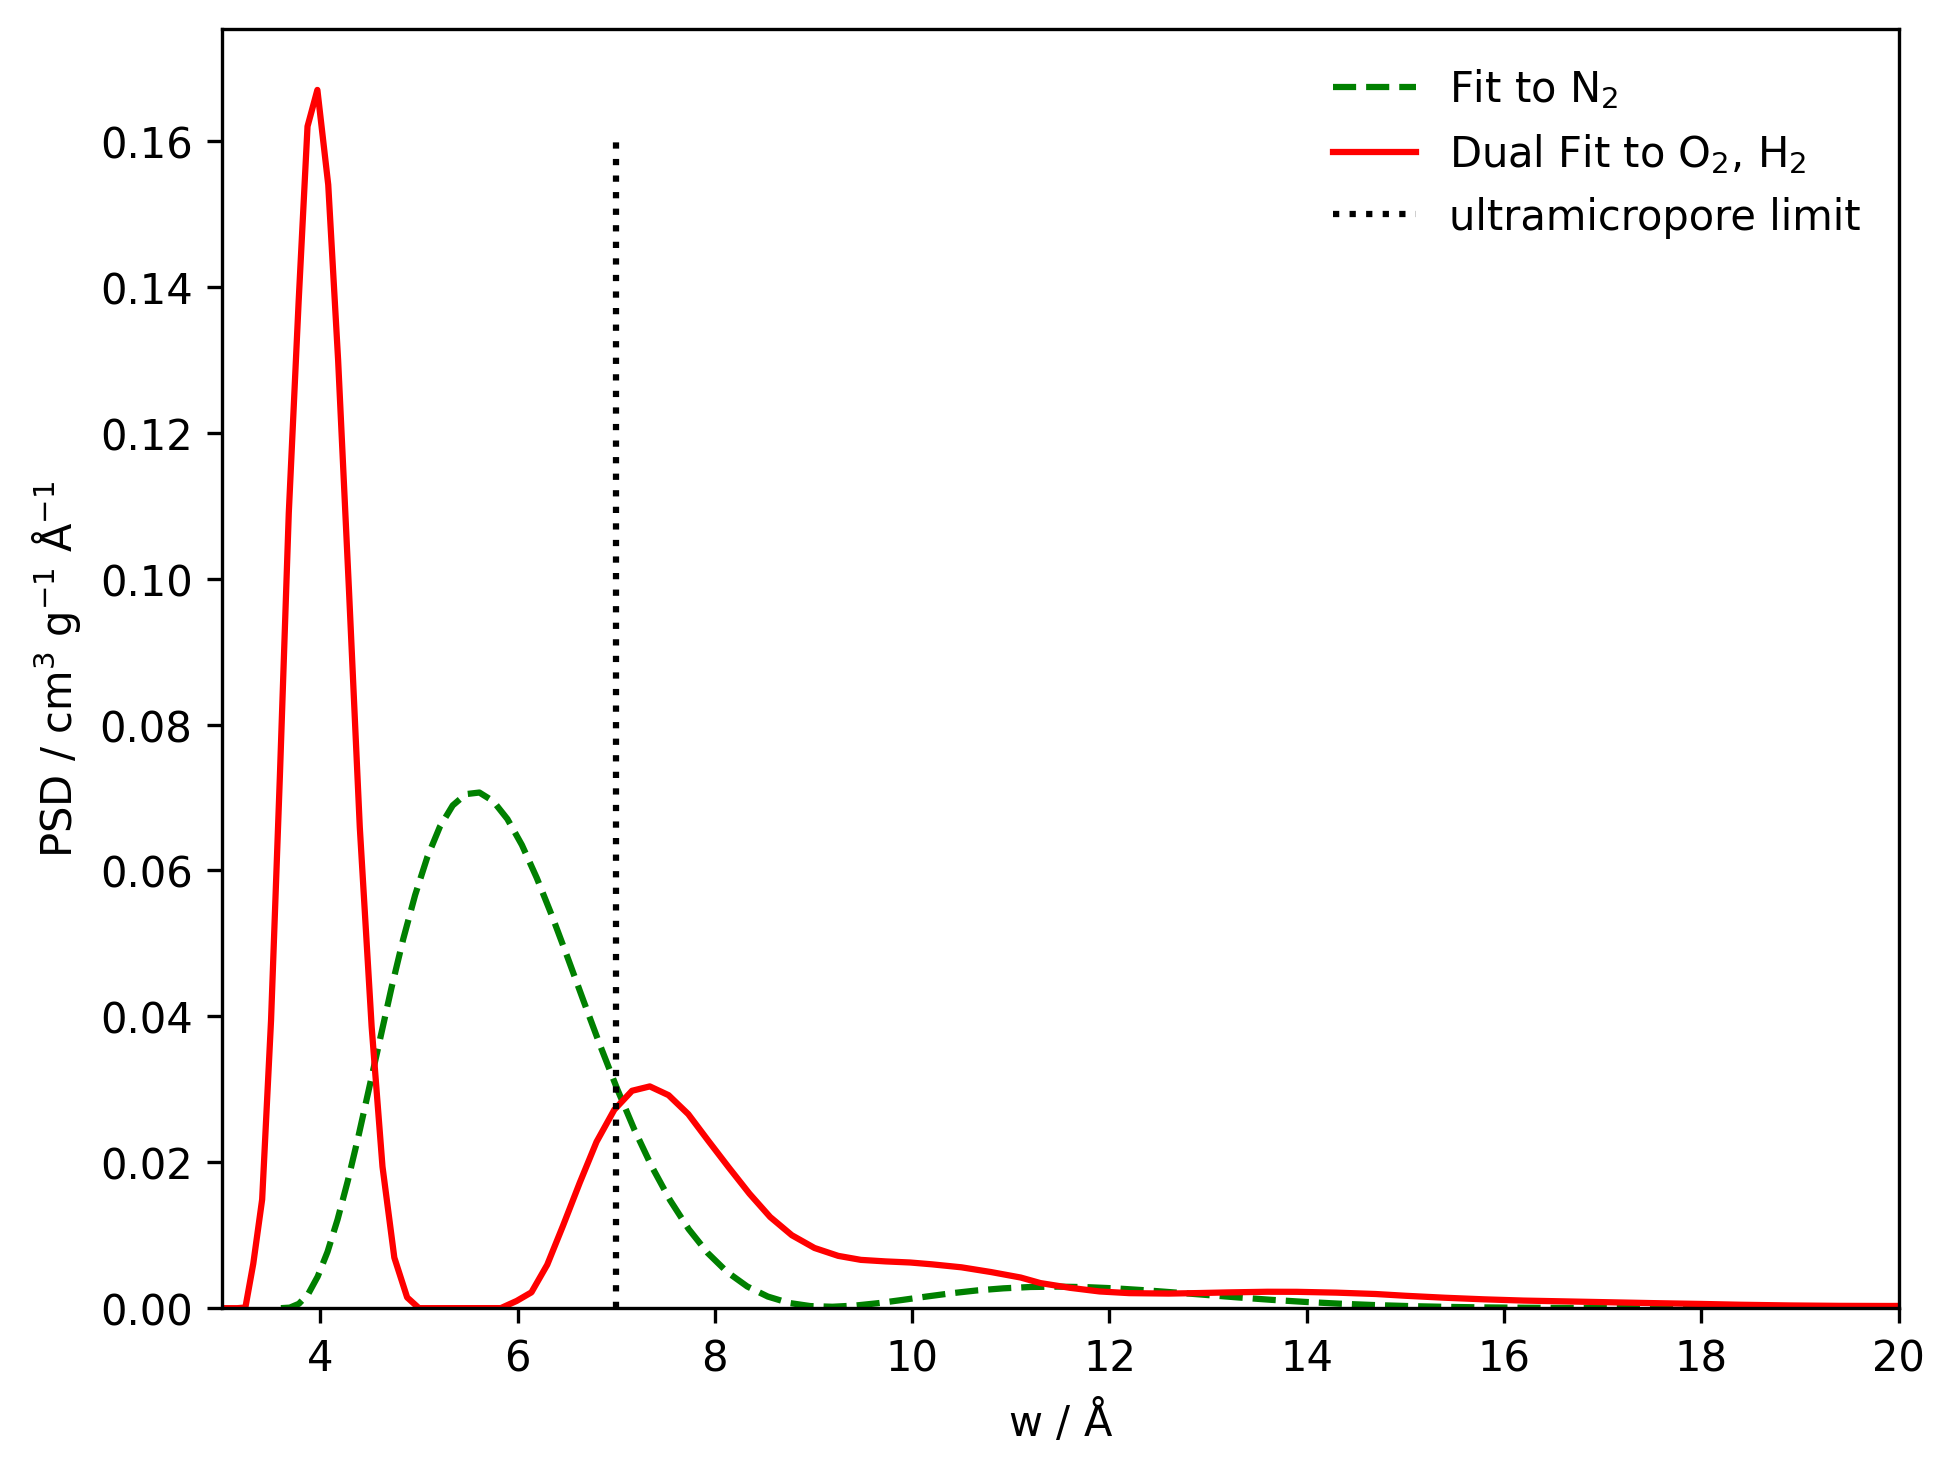
\includegraphics[width=\columnwidth, keepaspectratio]{5-dual_isotherm/figs/dual_psd_compare.png}
    \captionof{figure}{An example of the different \acrshortpl{psd} from single fit to \ce{N2} and dual fit to \ce{O2} and \ce{H2} isotherms on sample SA0.00-250. The \gls{ultramicropore} limit is also shown; clearly the dual fit shows a separation in pore regions that is different to the \gls{ultramicropore} limit of \qty{7.0}{\angstrom}. \newline}
    \label{fig:dual_psd_compare}
    
    \captionof{table}{Pore volume ($V_{NLDFT}$) and surface area ($A_{NLDFT}$) of selected samples from chapters \ref{ch:cbs} and \ref{ch:impregnation} in the \gls{micropore} region, divided into two regions according to the local minimum ($w_{locmin}$). Porosities calculated with simultaneous fit of 2D-NLDFT-HS kernels to \ce{O2} and \ce{H2} isotherms.}
    \begin{tabularx}{\textwidth}{llXXXX}
    \toprule
        \textbf{Sample} & $\mathbf{w_{locmin}}$ \textbf{/ \unit[detect-weight]{\angstrom}} & \multicolumn{2}{c}{$\mathbf{V_{NLDFT}}$ \textbf{/ \unit[detect-weight]{\cm\cubed\per\gram}}} & \multicolumn{2}{c}{$\mathbf{A_{NLDFT}}$ \textbf{/ \unit[detect-weight]{\metre\squared\per\gram}}} \\
        & & \textbf{1} & \textbf{2} & \textbf{1} & \textbf{2} \\
    \midrule
        NC0.0-800 & 5.5 & 0.14 & 0.09 & 715 & 184 \\
        NC0.7-800 & 5.3 & 0.12 & 0.15 & 620 & 366 \\
        NC0.9-800 & 5.4 & 0.13 & 0.20 & 669 & 507 \\
        \\
        SA1.00-200 & 6.1 & 0.20 & 0.38 & 868 & 824 \\
        \\
        SA0.00-250 & 5.4 & 0.12 & 0.33 & 627 & 811 \\
        SA0.50-250 & 6.1 & 0.17 & 0.35 & 812 & 820 \\
        SA1.00-250 & 6.1 & 0.19 & 0.37 & 841 & 195 \\
        \\
        hD-0700\textit{(1)} & 5.7 & 0.10 & 0.10 & 464 & 217 \\
        hD-0700\textit{(2)} & 5.5 & 0.09 & 0.09 & 444 & 217 \\
    \bottomrule
    \end{tabularx}
    \label{tb:finepore}
\end{figure}

The proportion of \glspl{micropore} taken up by these lower width peaks (peak 1) varies, with $V_{NLDFT}$ ranging from \qtyrange[list-units=single]{27}{61}{\percent} and $A_{NLDFT}$ from \qtyrange[list-units=single]{44}{81}{\percent} (see table \ref{tb:finepore}). This variation appears to be inversely related to degree of activation and indeed is the topic of \ref{pub:dual_iso}. In the case of the NC\textit{x.x-TTT} and SA\textit{x.xx}-250 samples it is clear that the proportion of microporosity taken up by the initial peak falls precipitously with \gls{porogen}:precursor ratio. The consistency found between the two repeats of hD-0700 (see table \ref{tb:n2_o2_classical}) when using \ce{O2} to determine classical measures of porosity is also present with these dual isotherm 2D-NLDFT-HS analyses. This lends further credence to the notion that the dual isotherm porosimetric method explored here may be superior to current, single isotherm methods.

The finer detail attained in the derived \acrshortpl{psd} from the dual \ce{O2}/\ce{H2} fits is of great interest as \glspl{ultramicropore} have been attributed to the low pressure uptake of \glspl{adsorbate} such as \ce{CO2} and \ce{H2}.\citep{Presser2011Effect, Sevilla2014Energy, Cabria2007optimum, DelaCasaLillo2002Hydrogen, Masika2012Hydrogen} What has not yet been investigated is the comparison of dual \ce{N2}/\ce{H2} fits with \ce{O2}/\ce{H2}. This, therefore is investigated in \ref{pub:dual_iso}. Furthermore, the work in chapter \ref{ch:pyPUC} shows that the porosity as shown by these dual isotherm techniques does have physical significance at least in terms of \ce{CO2} uptake capacity.
%
\newpage
\section[Publication II]{Publication II: Confirmation of pore formation mechanisms in biochars and activated carbons by dual isotherm analysis}

\textbf{Contribution of the author}: The author performed all synthesis and instrumental analysis of samples in the work, analysed the results and wrote the manuscript.

\textbf{Note}: For this publication, the sample names are slightly different. The variable \textit{x.xx} in SA\textit{x.xx-HHH} samples is truncated to \textit{x.x}, i.e. SA0.5-250 in the publication is equivalent to SA0.50-250 in chapter \ref{ch:impregnation}. As for NC\textit{x.x-TTT} samples only samples with \textit{TTT} of \qty{800}{\degreeCelsius} are examined, thus NC0.9 is identical to NC0.9-800 in chapter \ref{ch:impregnation}.  

\setcounter{opagenum}{\thepage}
\newpage

\setlength{\originalVOffset}{\voffset}   
\setlength{\originalHOffset}{\hoffset}

\setlength{\voffset}{0cm}
\setlength{\hoffset}{0cm}
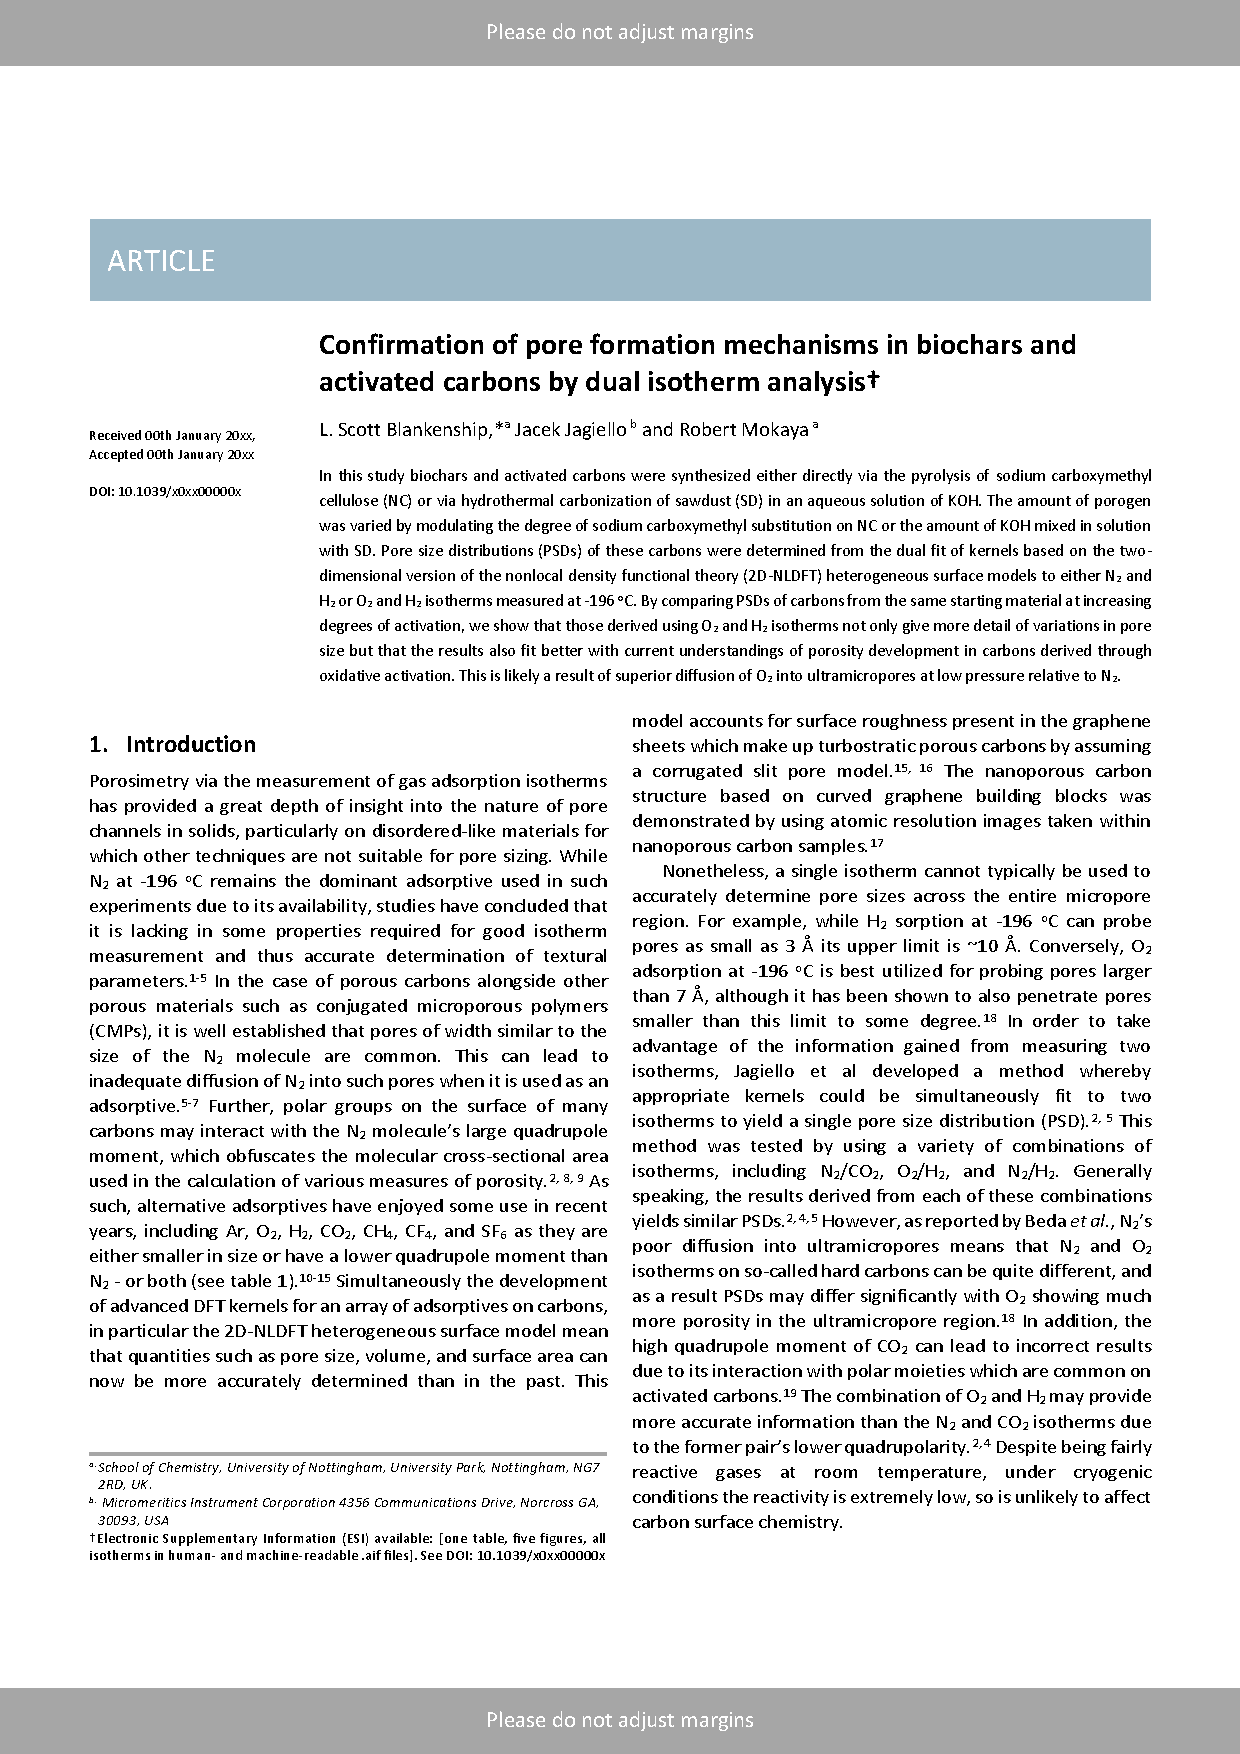
\includepdf[pagecommand={
    \setcounter{page}{\theopagenum}
    \thispagestyle{empty}
    },
    pages=-]{5-dual_isotherm/publication_02.pdf}
\setlength{\voffset}{\originalVOffset}
\setlength{\hoffset}{\originalHOffset}

\newpage
\section{Further analysis}
\ref{pub:dual_iso} contains only the \acrshortpl{psd} from the analysis of the SA\textit{x.xx}-250 and SA\textit{x.xx}-300 series as well as NC\textit{x.x}-800 series for \textit{x.x} in the range 0.0 to 0.9. Since publication, dual isotherm analyses of SA0.50-200, SA1.00-200 and NC1.2-800 has been completed. A discussion of the results follows here, particularly in relation to the utility of dual isotherm analyses on monitoring \acrshort{psd} development with changes in sample preparation conditions.

\subsection{Effect of hydrothermal impregnation temperature on porosity development in SD samples}

As discussed in section \ref{ss:sd_results}, the classically derived porosities of samples synthesised from \acrfull{sd} with identical \ce{KOH}:\acrshort{sd} ratios, do not vary significantly with \acrshort{htc} temperature. Nonetheless, it is interesting to compare such results using different porosimetric techniques. The \acrshortpl{psd} and associated fits are displayed in the appendix, figures \ref{fig:SA050-xxx_isopsd}, \ref{fig:SA100-xxx_isoposd}. While the dual \ce{O2}/\ce{H2} fits do appear to show small shifts in the position of the second maximum in the \acrshort{psd} for SA0.50-\textit{HHH} samples with hydrothermal impregnation temperature (see figure \ref{fig:SA050-xxx_isopsd}(2P)), this is not evident for SA1.00-\textit{HHH} samples (figure \ref{fig:SA100-xxx_isoposd}(2P)). Indeed it could be concluded that the dual \ce{N2}/\ce{H2} fits show just as much variation in the position of the second maximum. Thus, the \acrshort{psd} broadening observed in \ref{pub:dual_iso} according to dual isotherm \ce{O2}/\ce{H2} analysis is apparently only associated with \ce{KOH}:\acrshort{sd} ratio, as opposed to hydrothermal impregnation temperature.

\begin{figure}[hb!]
    \centering
    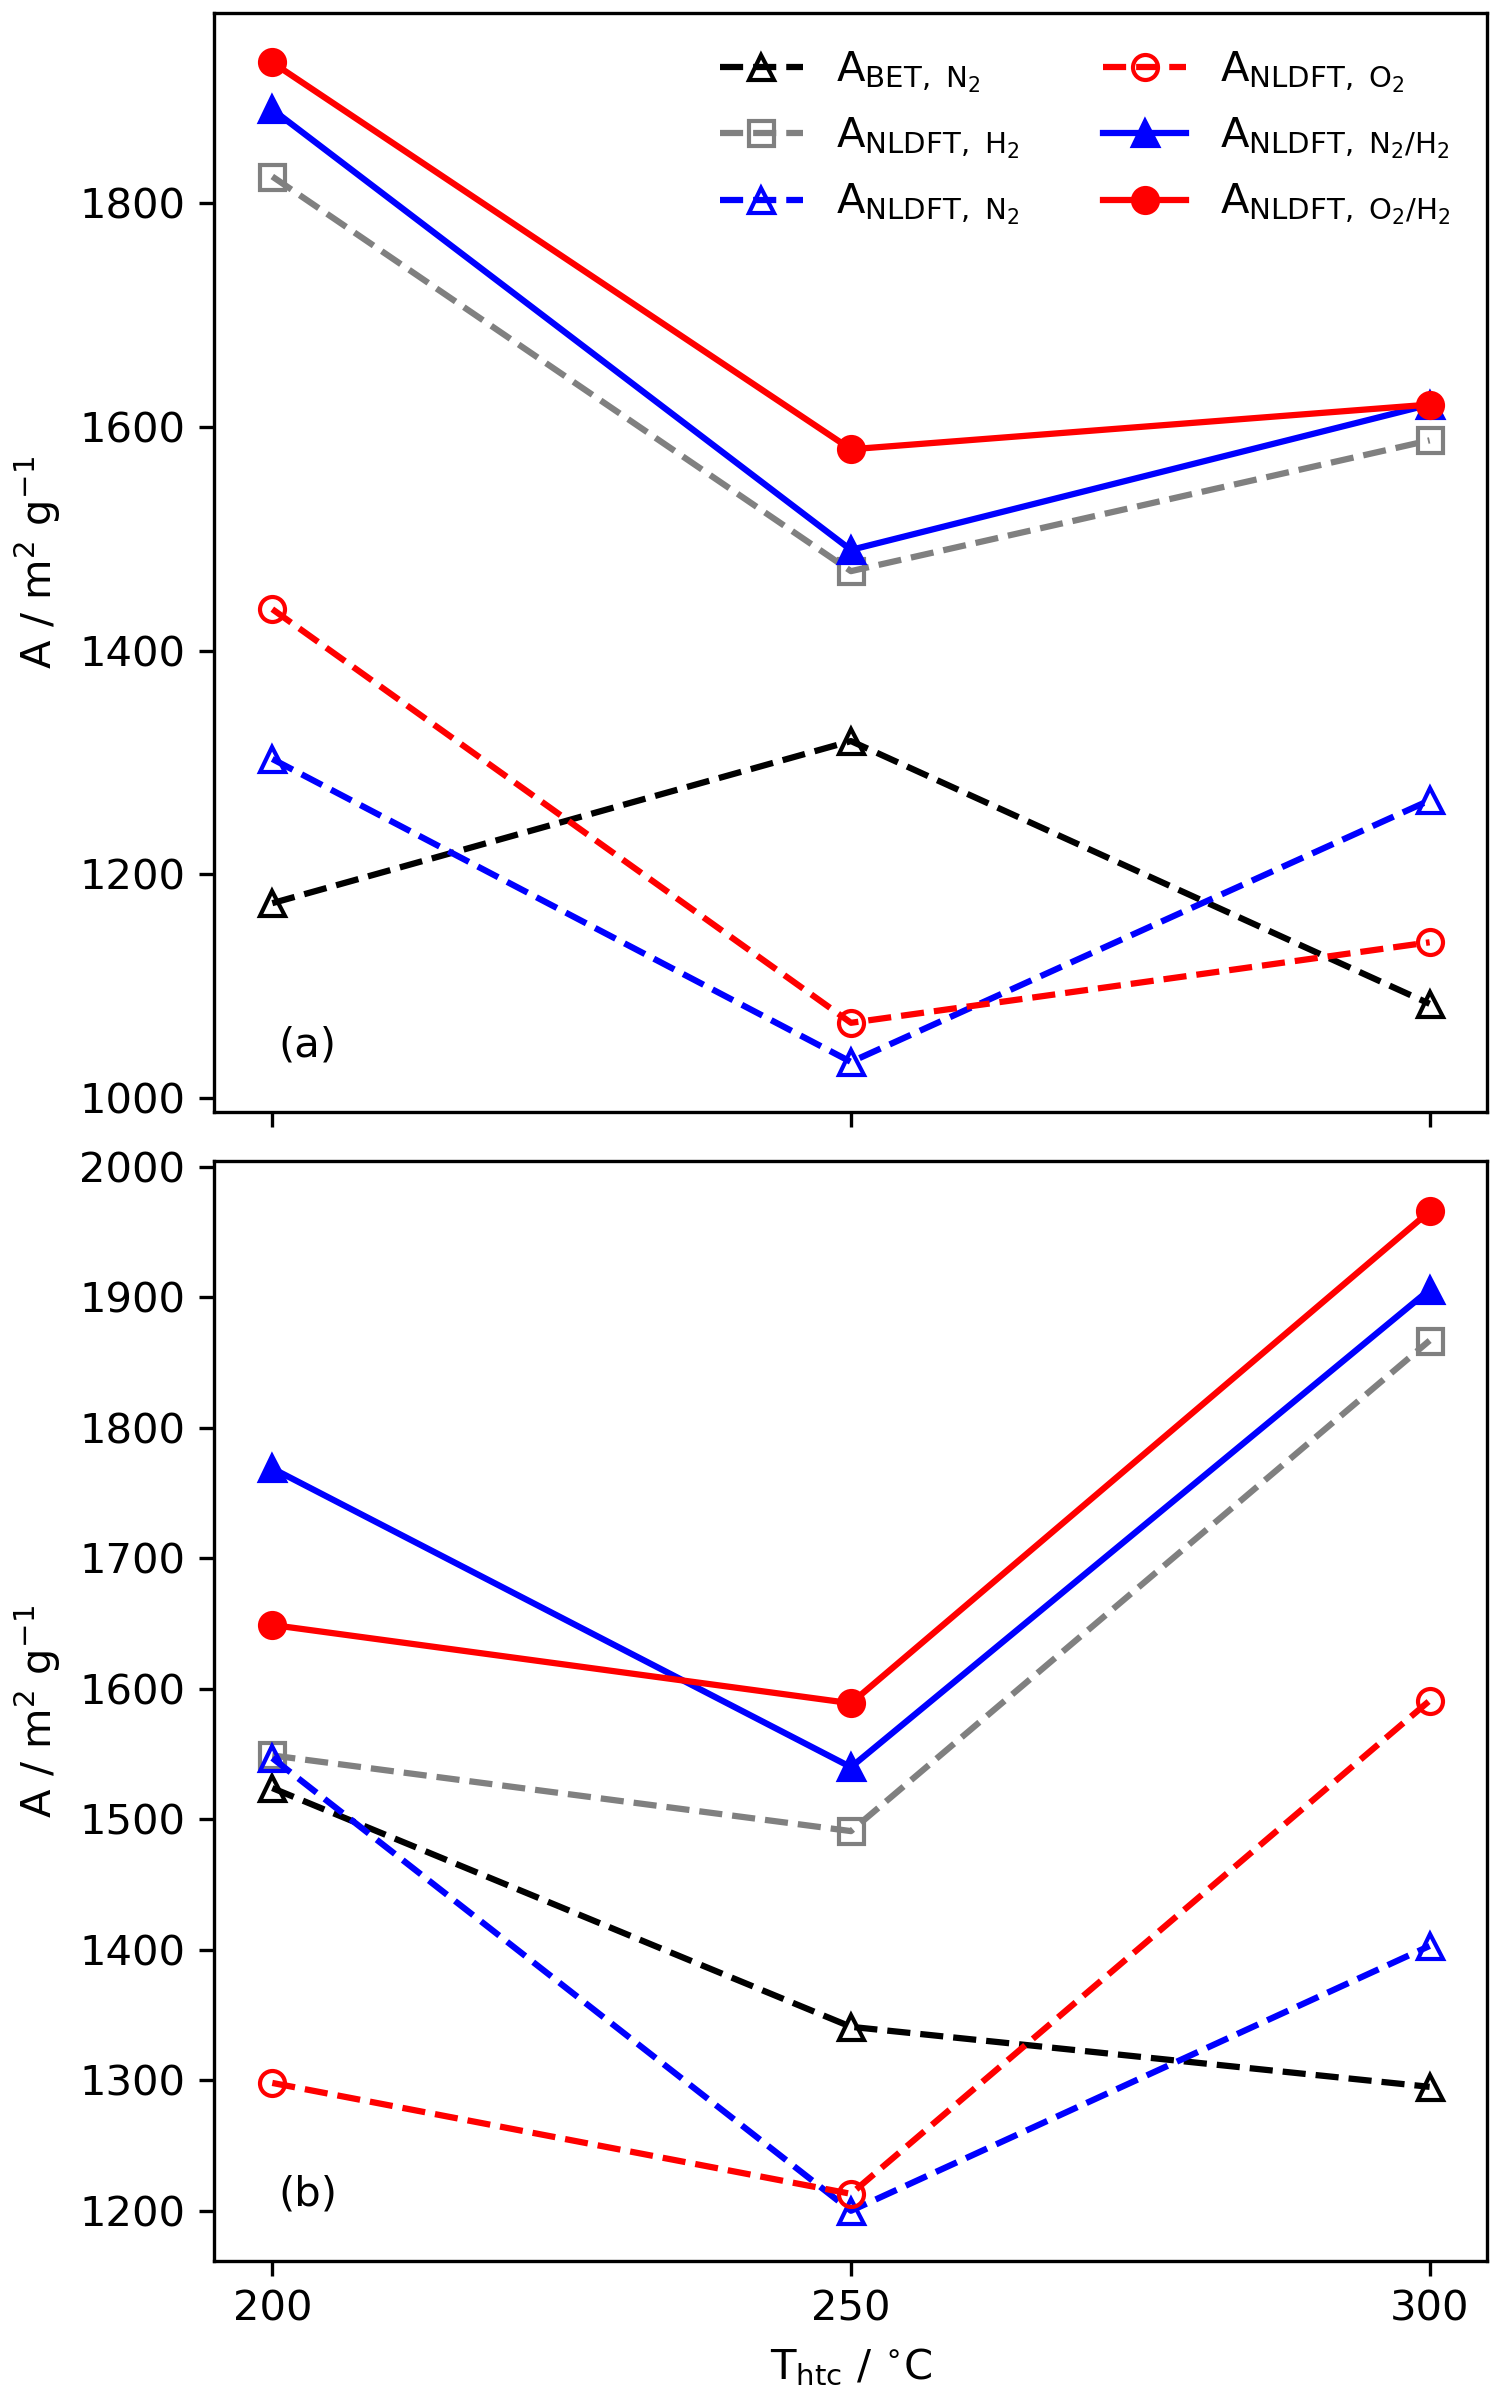
\includegraphics[width=0.7\columnwidth,keepaspectratio]{5-dual_isotherm/figs/SD_classical_nldft.png}
    \caption{Trends in surface area with hydrothermal impregnation temperature $T_{htc}$ of \acrshort{sd}-derived carbons, as determined \textit{via} the BET method as well as from fitting of 2D-NLDFT-HS kernel to \ce{H2}, \ce{N2}, \ce{O2} isotherms as well as dual-fitting to \ce{N2}/\ce{H2} and \ce{O2}/\ce{H2} pairs. Subfigures (a) and (b) are for \ce{KOH}:\acrshort{sd} ratios of 0.50 and 1.00 respectively.}
    \label{fig:classical_nldft_compare}
\end{figure}

A comparison of the trends in apparent surface area with hydrothermal carbonisation temperature ($\rm T_{htc}$) as determined by the \acrshort{bet} method on an \ce{N2} isotherm,\citep{Brunauer1938Adsorption} as well as \textit{via} fitting of 2D-NLDFT-HS kernels to \ce{N2}, \ce{O2}, \ce{H2} isotherms and dual fitting to \ce{N2}/\ce{H2}, \ce{O2}/\ce{H2} pairs is shown in figure \ref{fig:classical_nldft_compare}. For samples derived with both \ce{KOH}:\acrshort{sd} ratios of 0.50 and 1.00, the 2D-NLDFT method consistently shows a minimum in apparent surface area at $T_{htc}$ of \qty{250}{\degreeCelsius}. This is in contrast to $A_{BET,N_2}$ which shows a \textit{maximum} at this temperature for \ce{KOH}:\acrshort{sd} of 0.50, and a consistent decrease with temperature when the ratio is 1.00. Thus this discrepancy in the trend is likely a result of the inadequacy of the BET method for determining surface area in microporous materials, rather than an artefact of the nature of \ce{N2} \gls{adsorption}. Namely, the BET method relies on the formation of a monolayer in order to accurately quantify surface area, which is not possible in \glspl{micropore} as the probe molecule kinetic diameter is of the same order as the distance between pore walls (i.e. the pore width, $w$).\citep{Rouquerol2007Is, coasne2004grand, ambroz2018evaluation, walton2007applicability} Furthermore, the nature of the \gls{adsorption} is uncertain, as it is unknown to what degree the probe molecule is adsorbed on each of the pore walls in the (apparently) slit-shaped pores.\citep{Rouquerol2007Is, Brunauer1938Adsorption} \acrshort{nldft}-derived porosity, and in particular surface area determination does not have these assumptions that are unsuitable for highly microporous materials. Indeed, the kernel of model isotherms used in the 2D-NLDFT-HS method\citep{Jagiello20132D} is specifically designed for and suited to this kind of material. 

Of further interest are the relative apparent surface areas determined by each probe molecule using the 2D-NLDFT-HS method. \ce{O2} and \ce{N2} single fits give approximately similar values and are in a similar range as those derived using $A_{BET}$. Simultaneously dual isotherm \ce{O2}/\ce{H2} and \ce{N2}/\ce{H2}, as well as single isotherm \ce{H2} derived areas match well with one another, but give significantly higher values than the previously mentioned methods. This further confirms that the use of \ce{H2} as a probe molecule allows for the penetration of pores inaccessible to the larger \ce{O2} and \ce{H2} as was mentioned in \ref{pub:dual_iso}. The similarity in apparent surface areas derived using \ce{H2} alone, with the dual fit methods for a \ce{KOH}:\acrshort{sd} ratio of 0.50 is striking, indicating that all relevant porosity is accessible by \ce{H2} for these materials. There is greater discrepancy when \ce{KOH}:\acrshort{sd} is increased to 1.00, probably a result of \acrshort{psd} broadening through more aggressive action of the \gls{porogen}, and thus creating porosity accessible to \ce{N2} or \ce{O2} but which will not be filled by \ce{H2} at pressures up to \qty{1}{\bar}.

\subsection{\texorpdfstring{\acrshort{psd} contraction in NC samples}{PSD contraction in NC samples}}

In section \ref{ss:NC}, a surprising reduction in total porosity for \textit{x.x} of 1.2 was discussed. That is, while increasing the \acrfull{ds} of \ce{Na} from 0.7, to 0.9 porosity increases ($A_{BET}$ and $V_t$), but these metrics reduce again when \acrshort{ds} is increased further to 1.2 (see table \ref{tb:nc_porosity}). This drop in overall porosity is also accompanied by small reductions in \% microporosity, and the trend occurs regardless of activation temperature. The more advanced techniques detailed in this chapter should give more detail as to the changes in porosity, and as such the \acrshortpl{psd} and associated isotherms and fits are shown in figure \ref{fig:NC_contraction}. This is of course a reproduction of \textbf{figure 3} in \ref{pub:dual_iso}, but with the inclusion of NC1.2-800 (referred to as NC1.2 in the publication).  

\begin{figure}[ht!]
    \centering
    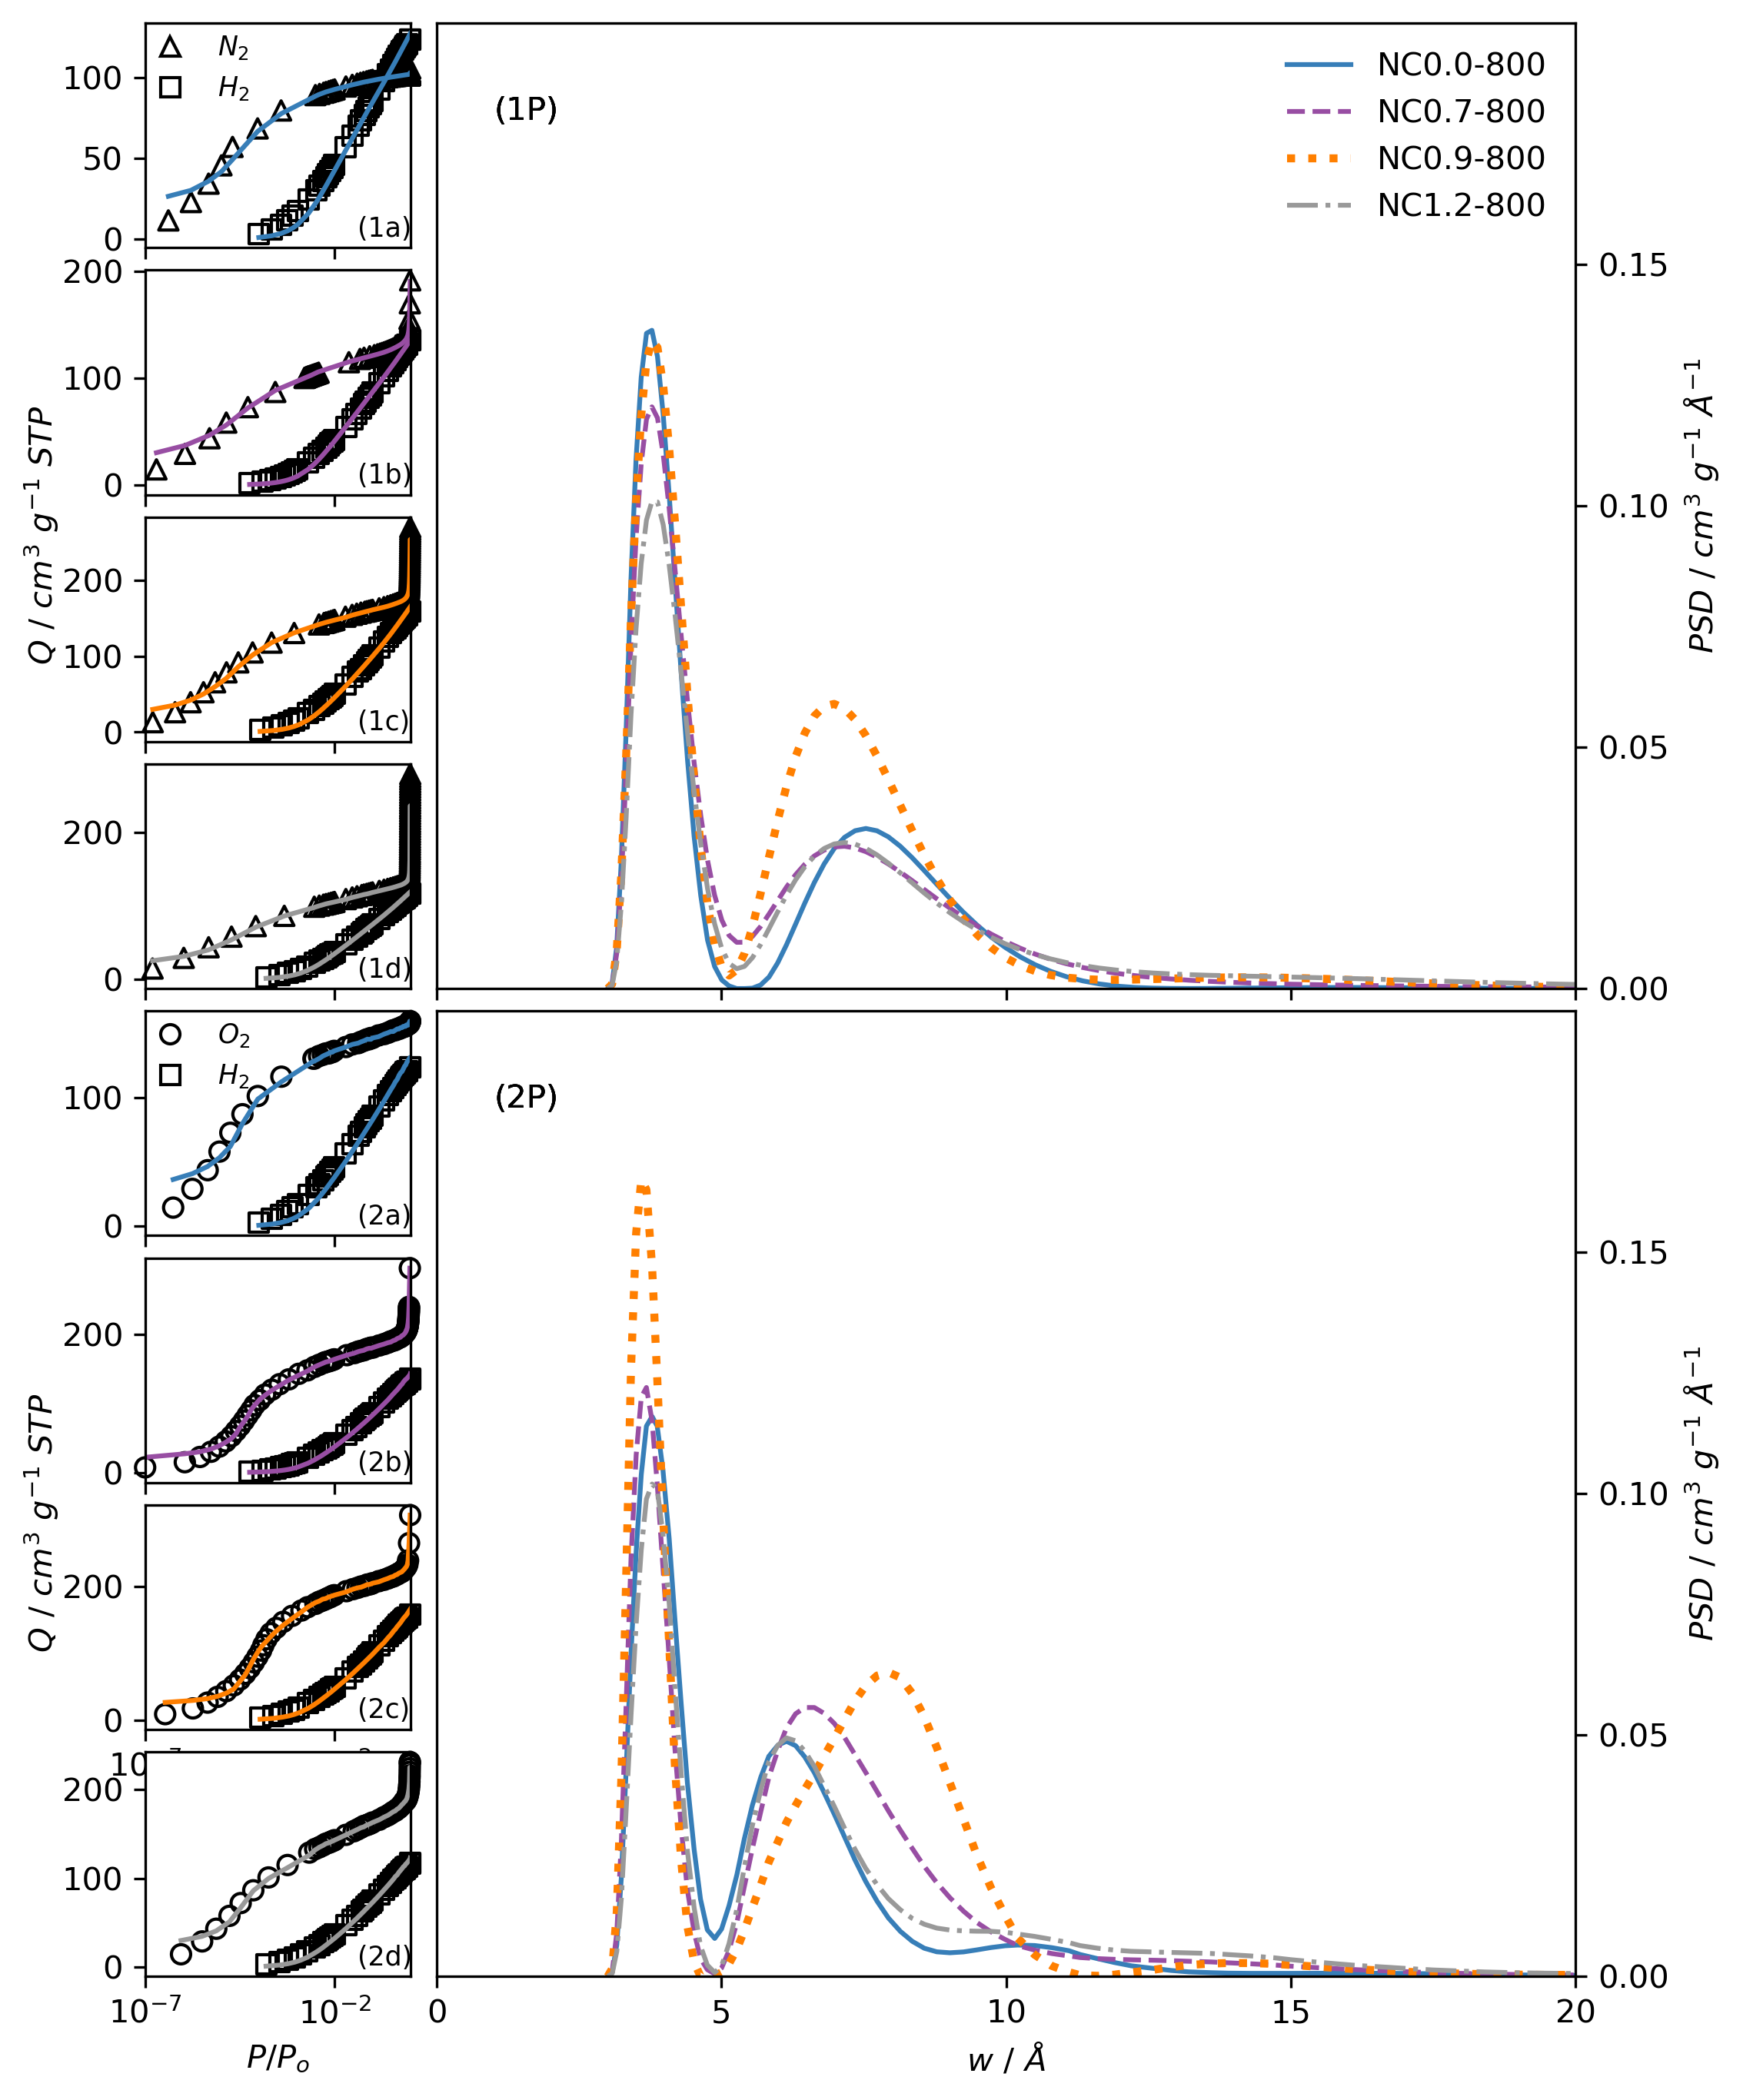
\includegraphics[width=\columnwidth,keepaspectratio]{5-dual_isotherm/figs/NCdual_isopsd.png}
    \caption{Fits to \ce{N2}/\ce{H2} (1a, 1b, 1c) and \ce{O2}/\ce{H2} (2a, 2b, 2c) isotherms of samples NC\textit{x.x}-800 (for all values of \textit{x.x} from 0.0 to 1.2), and resultant \acrshortpl{psd} (1P, 2P).}
    \label{fig:NC_contraction}
\end{figure}

The analysis performed using dual \ce{N2}/\ce{H2} porosimetry (see figure \ref{fig:NC_contraction}(1P)) indicates that the reduction in porosity for NC1.2-800 is associated with a decrease in the size of the peaks in the \acrshort{psd} relative to NC0.9-800. That is, there is no significant shift in in the position of the maxima but simply a reduction in overall porosity associated with both of these maxima. This is consistent with the overall conclusion in \ref{pub:dual_iso}, in that \ce{N2}/\ce{H2} analysis doesn't show variation in pore widths with degree of activation. On the other hand, \ce{O2}/\ce{H2} analysis (see figure \ref{fig:NC_contraction}(2P)) shows a contraction in the breadth of the \acrshort{psd} for \textit{x.x} of 1.2. Indeed, the position of the second maximum is the same as that for NC0.0-800. 

In section \ref{ss:NC} it was suggested that the trends in porosity were a result of competitive pore forming processes; while pore formation was dominated by formation of cross-links at \acrshort{ds} of 0.7 and 0.9, oxidative chemical activation began to take on a larger role at \acrshort{ds} of 1.2. In the case of NC0.0-800, no cross-link formation can occur thus porosity is formed \textit{via} gasification. The contraction in \acrshort{psd} for NC1.2-800 shown by \ce{O2}/\ce{H2} analysis indicates that this higher quantity of \ce{Na} present during \gls{pyrolysis} results in the destruction of cross-links and thus of the broader pores that are associated with their formation. The porosity that remains is that formed solely \textit{via} gasification as present in the \ce{Na}-free samples. On the other hand, the information given by \ce{N2}/\ce{H2} analysis indicates that there is a loss in porosity that is much more mechanistically difficult to explain. Perhaps the reduction in size of the second maximum could simply be put down to of pore collapse \textit{via} overactivation, but this ought to be associated with much more significant increase in mesoporosity which is not present here. It is much more difficult to derive nuanced, logical hypotheses on these pore formation mechanisms from the \ce{N2}/\ce{H2} analysis.

\section{Summary \& future work}
Porosimetry performed using \ce{O2} shows promise in more accurate determination of \acrshort{psd}, and porosity in general in ultramicroporous carbons. In particular, simultaneous fitting of the respective 2D-NLDFT-HS kernel to \ce{O2} and \ce{H2} isotherms consistently reveals a bimodal \acrshort{psd}. While this is also present for dual fits to \ce{N2} and \ce{H2}, the \ce{O2}/\ce{H2} method seems to show broadening in the \acrshort{psd} with increasing degree of activation which is not present in analysis performed using the former pair. These results ought to inform the selection of porosimetric \glspl{adsorbate} for highly ultramicroporous carbons. Furthermore, the results from dual isotherm analyses give further insights into potential mechanistic details of the somewhat unusual pore formation mechanisms in the \glspl{turbostratic carbon} reported in chapter \ref{ch:impregnation}. 

There was an attempt to fit three isotherms (\ce{N2}, \ce{O2}, and \ce{H2}) to their respective 2D-NLDFT-HS kernels simultaneously which proved fruitless. This gave poor fits to the experimental data, especially for carbons with a low degree of activation. As stated in \ref{pub:dual_iso}, \textbf{section 4.} this may indicate the difficulty \ce{N2} has in penetrating the smallest of \glspl{ultramicropore} and thus its limited utility in measuring porosity at these pore widths. However, three-way fits may indeed prove to be useful in the future in particular for materials with greater \acrshort{psd} hierarchy. For example, a simultaneous fit to \ce{SF6}, \ce{O2} and \ce{H2} isotherms (at \qtylist[list-units=single]{-50;-196;-196}{\degreeCelsius} respectively) would minimise the overlap of accessible pores for each of the three \glspl{adsorbate}, as the $d_k$ is \qty{5.50}{\angstrom}, so excludes the smallest of \glspl{ultramicropore}. This analysis may however not be necessary and the same information could be gleaned by using \ce{SF6} and \ce{H2}, which would minimise the overlap of pore sizes accessible to both \glspl{adsorbate} In addition, \ce{SF6} has a zero quadrupole moment compared to \ce{O2}'s of 0.155 which ought to reduce errors produced by carbon surface heterogeneity.


\newpage
\section[Publication II Supporting Information]{Publication II Supporting Information: Confirmation of pore formation mechanisms in biochars and activated carbons by dual isotherm analysis}

\textbf{Contribution of the author}: The author performed all synthesis and instrumental analysis of samples in the work, analysed the results and wrote the manuscript.

\textbf{Note}: For this publication, the sample names are slightly different. The variable \textit{x.xx} in SA\textit{x.xx-HHH} samples is truncated to \textit{x.x}, i.e. SA0.5-250 in the publication is equivalent to SA0.50-250 in chapter \ref{ch:impregnation}. As for NC\textit{x.x-TTT} samples only samples with \textit{TTT} of \qty{800}{\degreeCelsius} are examined, thus NC0.9 is identical to NC0.9-800 in chapter \ref{ch:impregnation}.
\setcounter{opagenum}{\thepage}
\newpage

\setlength{\originalVOffset}{\voffset}   
\setlength{\originalHOffset}{\hoffset}

\setlength{\voffset}{0cm}
\setlength{\hoffset}{0cm}
% too big for overleaf, try compilation later.

\includepdf[pagecommand={
    \setcounter{page}{\theopagenum}
    \thispagestyle{empty}
    },
    pages=-]{5-dual_isotherm/si_02.pdf}
\setlength{\voffset}{\originalVOffset}
\setlength{\hoffset}{\originalHOffset}

\bibliographystyle{rsc}
\bibliography{bibliography/bib}

\begin{subappendices}
\newpage

\begin{figure}[hptb]
    \centering
    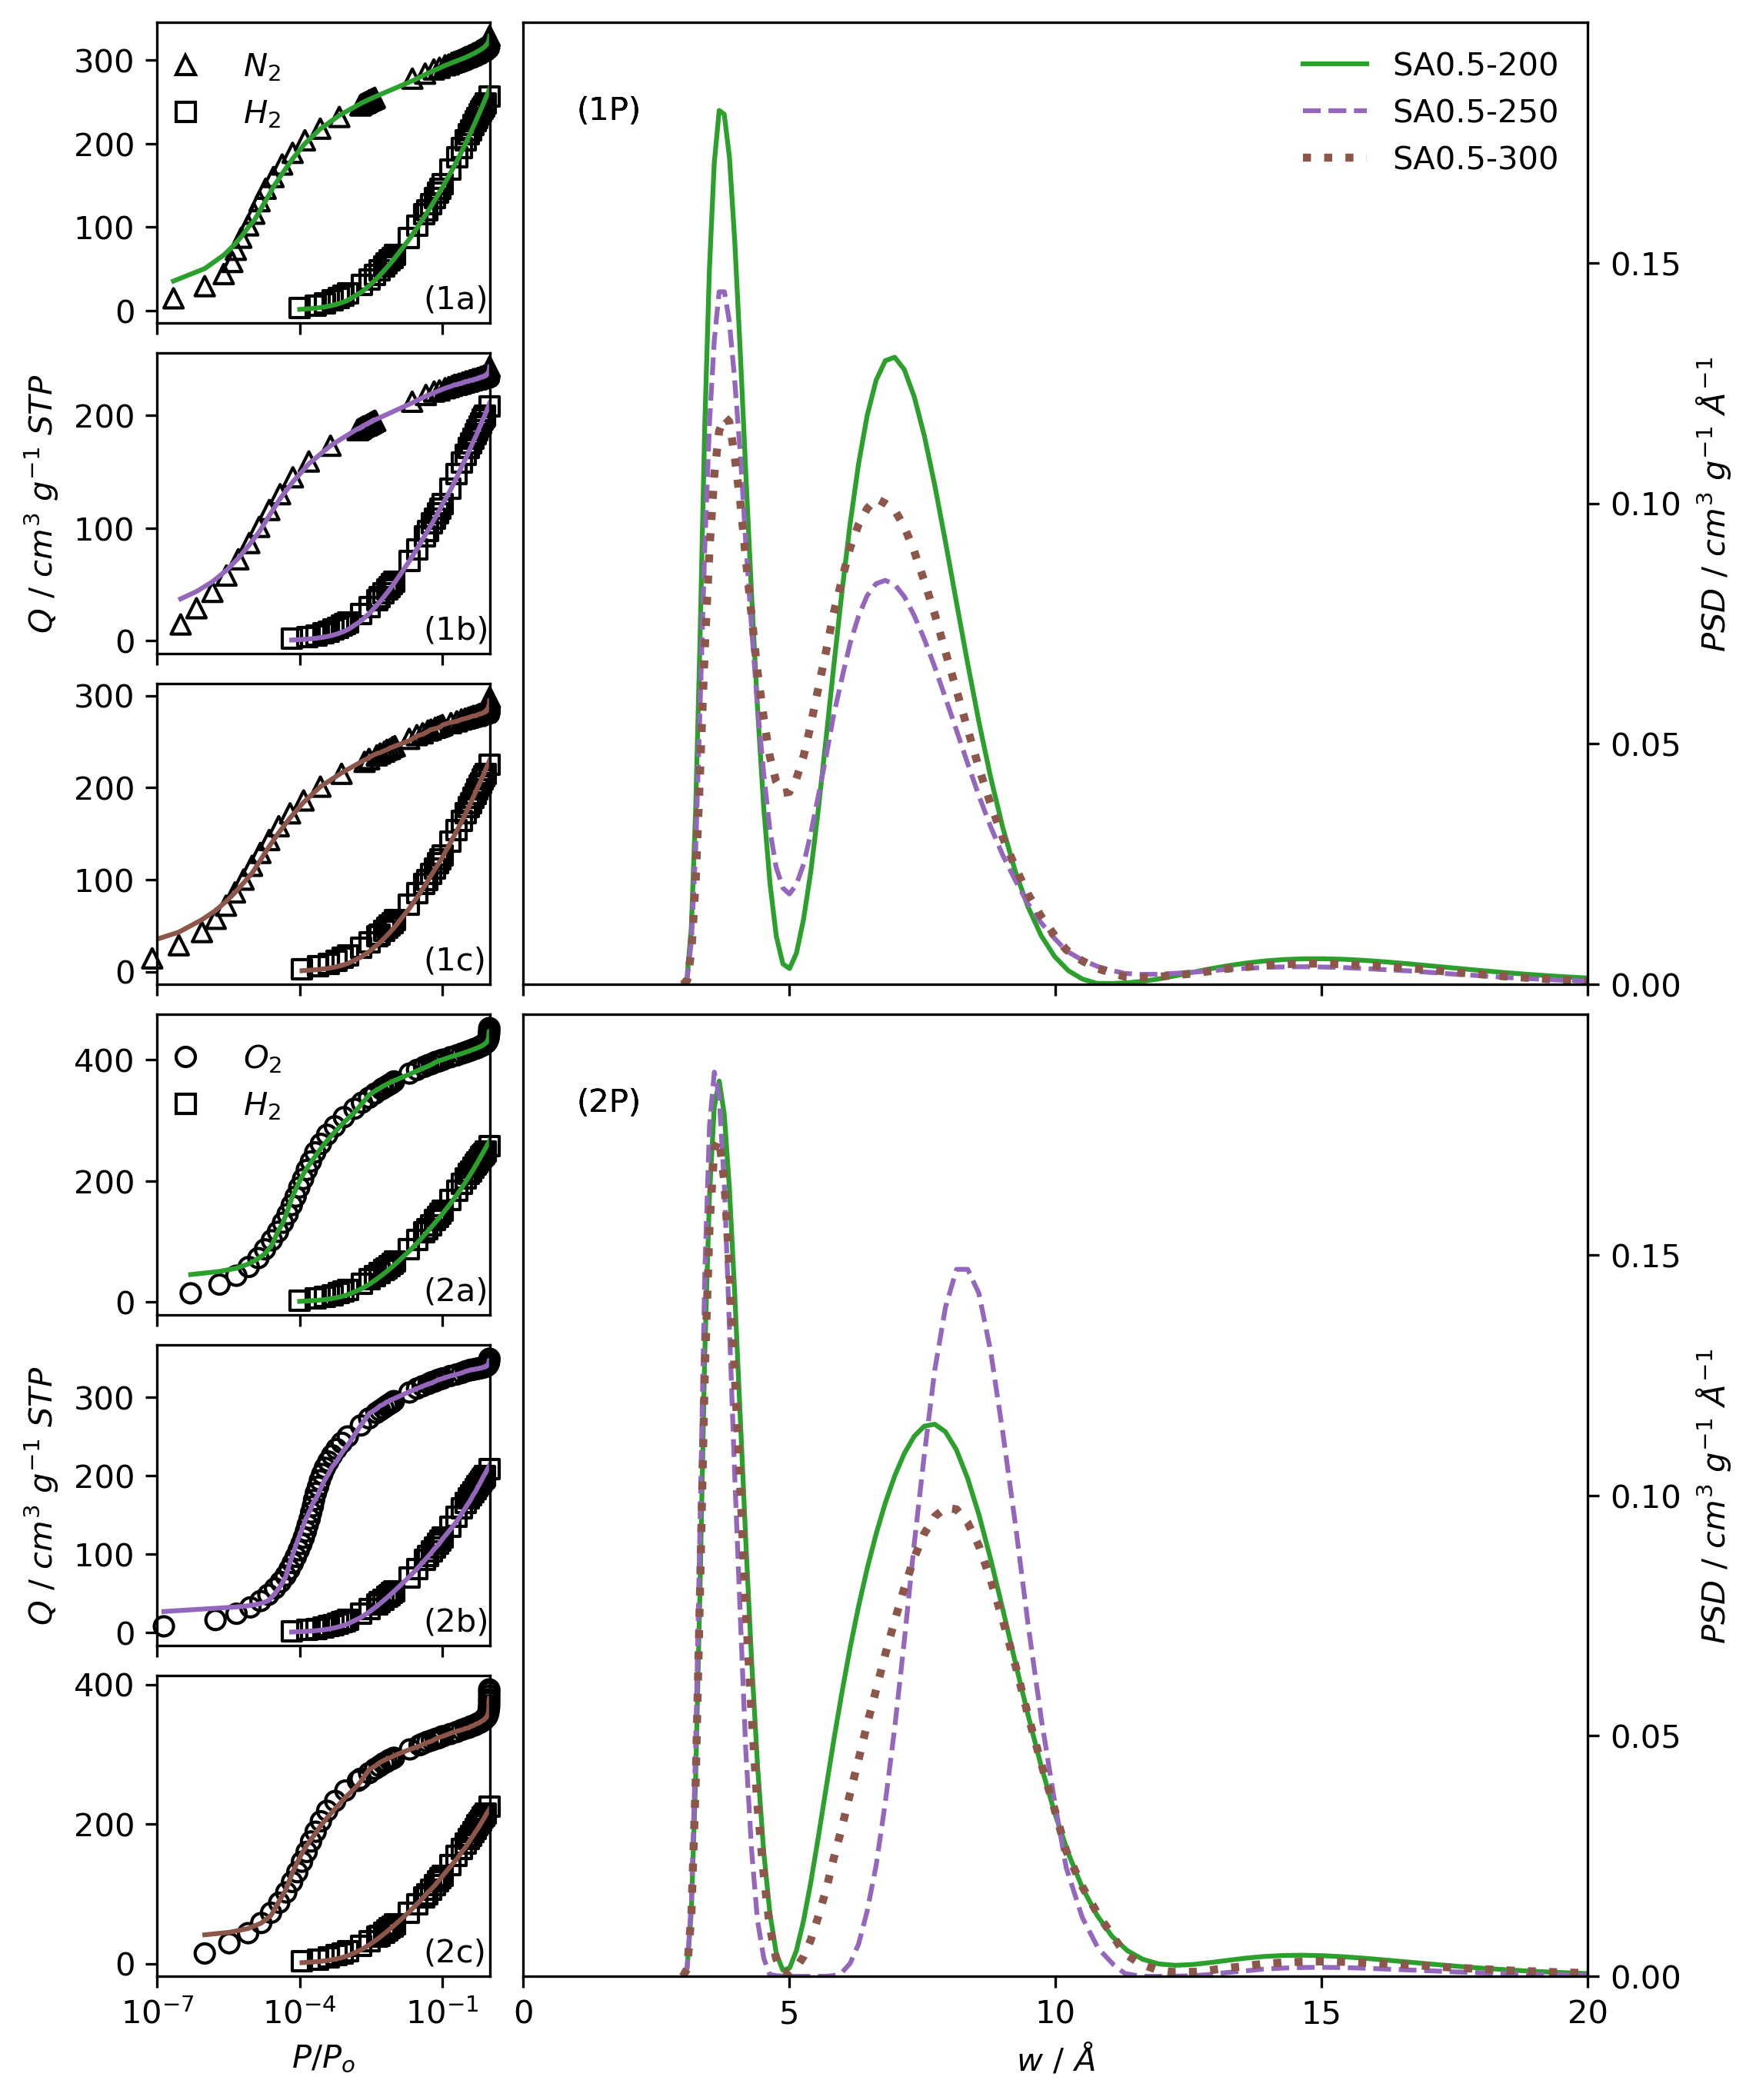
\includegraphics[width=\columnwidth, keepaspectratio]{5-dual_isotherm/figs/SA050-xxx_isopsd.png}
    \caption{Changes in porosity with \gls{htc} temperature for SA0.5-\textit{TTT} carbons. Compared according to dual fit \ce{N2}/\ce{H2} (1) and \ce{O2}/\ce{H2} (2) porosimetry.}
    \label{fig:SA050-xxx_isopsd}
\end{figure}

\begin{figure}[hptb]
    \centering
    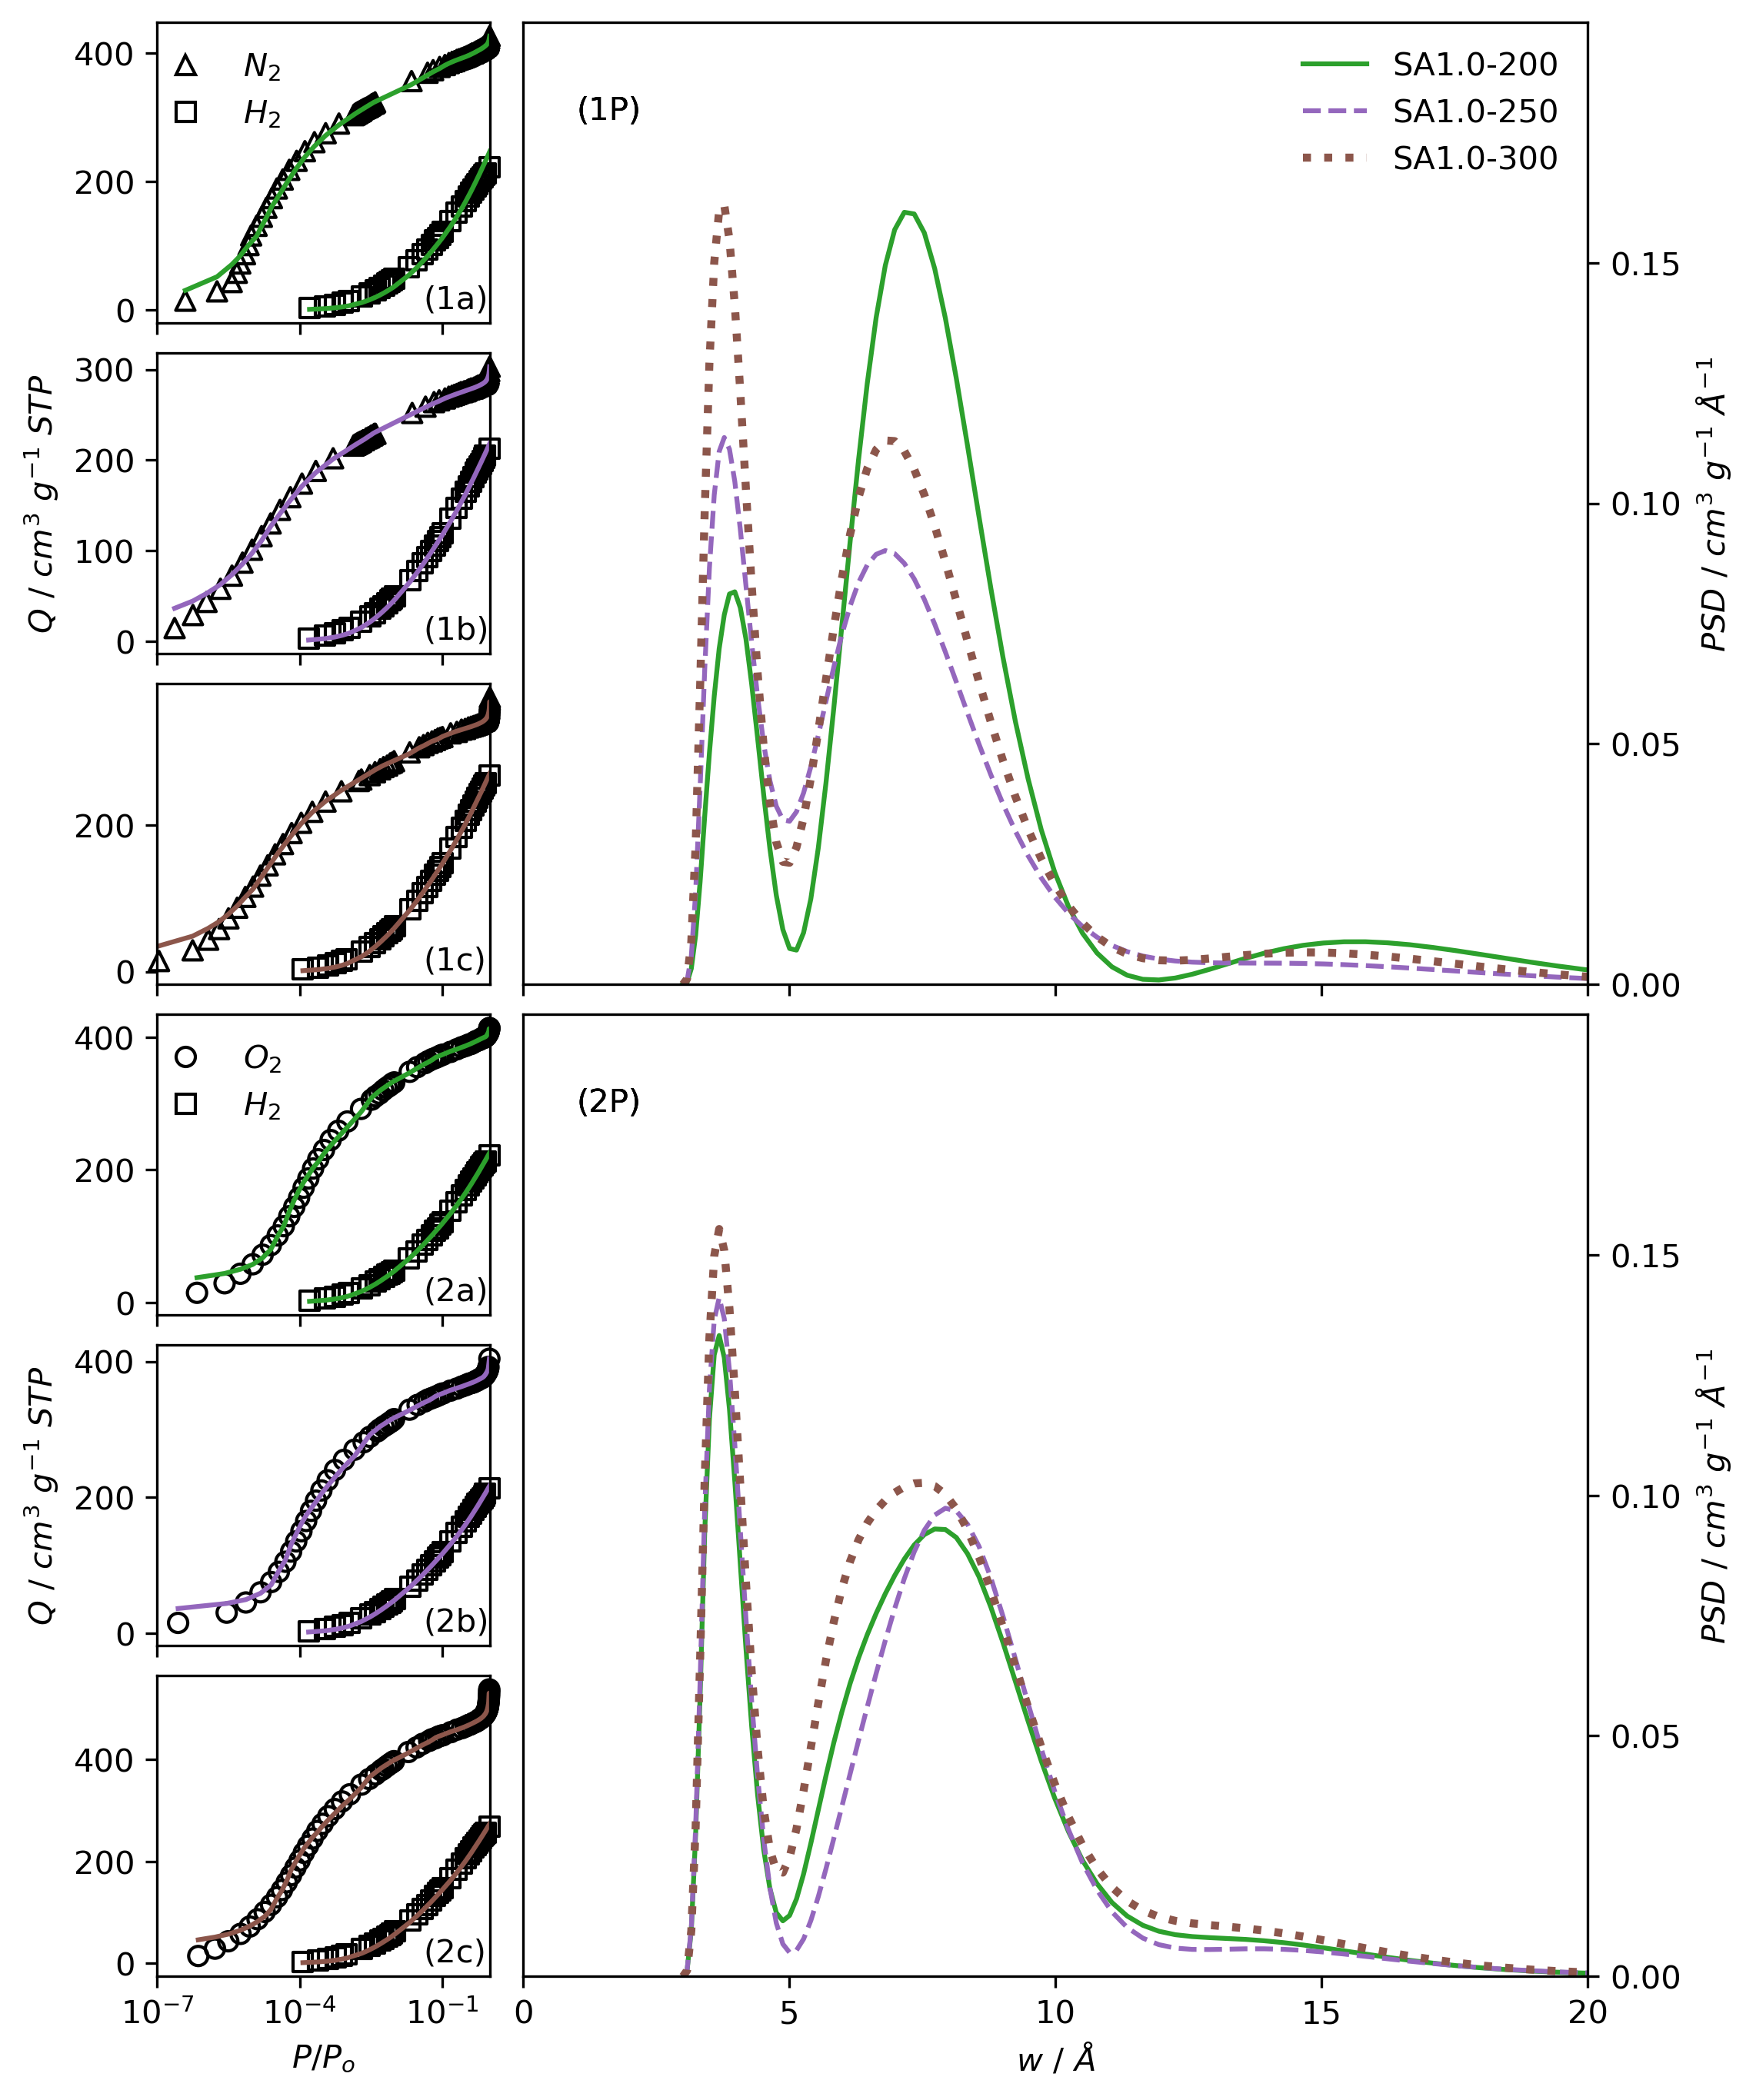
\includegraphics[width=\columnwidth, keepaspectratio]{5-dual_isotherm/figs/SA100-xxx_isopsd.png}
    \caption{Changes in porosity with \gls{htc} temperature for SA1.0-\textit{TTT} carbons. Compared according to dual fit \ce{N2}/\ce{H2} (1) and \ce{O2}/\ce{H2} (2) porosimetry.}
    \label{fig:SA100-xxx_isoposd}
\end{figure}
\end{subappendices}